% ============================================================
%  BÁO CÁO DỰ ÁN DATA SCIENCE
%  AirSense Hà Nội – Hệ thống Dự báo Chất lượng Không khí
%  Biên dịch với pdfLaTeX trên Overleaf
% ============================================================
\documentclass[12pt,a4paper]{report}

% ── Encoding & Language ─────────────────────────────────────
\usepackage[utf8]{inputenc}
\usepackage[T5]{fontenc}
\usepackage[vietnamese]{babel}

% ── Layout ──────────────────────────────────────────────────
\usepackage[top=2.5cm, bottom=2.5cm, left=3cm, right=2.5cm]{geometry}
\usepackage{setspace}
\setstretch{1.35}
\usepackage{parskip}
\setlength{\parindent}{0pt}

% ── Math ────────────────────────────────────────────────────
\usepackage{amsmath, amssymb, mathtools}

% ── Graphics & Colors ───────────────────────────────────────
\usepackage{graphicx}
\usepackage{xcolor}
\usepackage{colortbl}
\usepackage{tikz}
\usetikzlibrary{arrows.meta, shapes.geometric, positioning, calc}

% ── Tables ──────────────────────────────────────────────────
\usepackage{booktabs}
\usepackage{array}
\usepackage{tabularx}
\usepackage{longtable}
\usepackage{multirow}
\usepackage{makecell}

% ── Listings (code) ─────────────────────────────────────────
\usepackage{listings}
\lstset{
  basicstyle=\ttfamily\small,
  breaklines=true,
  frame=tb,
  language=Python,
  backgroundcolor=\color{gray!8},
  keywordstyle=\bfseries\color{blue!70!black},
  commentstyle=\itshape\color{gray!70},
  stringstyle=\color{orange!80!black},
  numbers=left,
  numberstyle=\tiny\color{gray},
  xleftmargin=1.5em,
  framexleftmargin=1.5em
}

% ── Caption & Figure ────────────────────────────────────────
\usepackage{caption}
\usepackage{subcaption}
\usepackage{float}
\captionsetup{font=small, labelfont=bf}

% ── Hyperlinks ──────────────────────────────────────────────
\usepackage{hyperref}
\hypersetup{
  colorlinks = true,
  linkcolor  = blue!70!black,
  citecolor  = blue!70!black,
  urlcolor   = blue!70!black
}

% ── Headers & Footers ───────────────────────────────────────
\usepackage{fancyhdr}
\pagestyle{fancy}
\fancyhf{}
\fancyhead[L]{\small\textit{AirSense Hà Nội -- Dự báo Chất lượng Không khí}}
\fancyhead[R]{\small\thepage}
\fancyfoot{}
\renewcommand{\headrulewidth}{0.4pt}

% ── Enum ────────────────────────────────────────────────────
\usepackage{enumitem}

% ── Custom Colors ───────────────────────────────────────────
\definecolor{cgood}{HTML}{2fbf71}
\definecolor{cmoderate}{HTML}{f2c94c}
\definecolor{csensitive}{HTML}{f2994a}
\definecolor{cunhealthy}{HTML}{eb5757}
\definecolor{cvery}{HTML}{9b51e0}
\definecolor{chazard}{HTML}{7b1f4d}
\definecolor{cblue}{HTML}{1a73e8}
\definecolor{headerblue}{HTML}{2c3e6b}

% ── Custom Commands ─────────────────────────────────────────
\newcommand{\good}[1]{{\color{cgood}\textbf{#1}}}
\newcommand{\warn}[1]{{\color{cmoderate}\textbf{#1}}}
\newcommand{\bad}[1]{{\color{cunhealthy}\textbf{#1}}}
\newcommand{\info}[1]{{\color{cblue}\textbf{#1}}}

% Chapter styling
\usepackage{titlesec}
\titleformat{\chapter}[display]
  {\normalfont\LARGE\bfseries\color{headerblue}}
  {\chaptertitlename\ \thechapter}{12pt}{\Huge\color{headerblue}}
\titlespacing*{\chapter}{0pt}{-10pt}{20pt}

% ============================================================
\begin{document}

% ── TRANG BÌA ───────────────────────────────────────────────
\begin{titlepage}
\centering
\vspace*{1cm}

{\large\textbf{TRƯỜNG ĐẠI HỌC [TÊN TRƯỜNG]}}\\[0.3cm]
{\large\textbf{KHOA CÔNG NGHỆ THÔNG TIN}}\\[0.3cm]
{\large\textbf{BỘ MÔN KHOA HỌC DỮ LIỆU}}

\vspace{1.5cm}

% Nếu có logo trường, thêm vào đây:
% \includegraphics[width=0.2\textwidth]{logo}

\vspace{0.8cm}

\rule{\linewidth}{2pt}\\[0.3cm]
{\Huge\bfseries\color{headerblue} AIRSENSE HÀ NỘI}\\[0.4cm]
{\LARGE\bfseries Hệ thống Dự báo Chất lượng Không khí\\theo Giờ sử dụng Machine Learning}\\[0.2cm]
\rule{\linewidth}{2pt}

\vspace{1cm}

\begin{minipage}{0.72\textwidth}
\centering
{\large \textbf{Báo cáo Đồ án Môn học: Khoa học Dữ liệu}}\\[0.6cm]
\begin{tabular}{ll}
\textbf{Nhóm thực hiện:} & Nhóm Data Science \\[3pt]
\textbf{Thành viên:}     & [Tên thành viên 1] \\
                          & [Tên thành viên 2] \\
                          & [Tên thành viên 3] \\[3pt]
\textbf{Giảng viên HD:}  & [Tên giảng viên] \\[3pt]
\textbf{Ngôn ngữ:}       & Python 3.11 \\
\textbf{Framework:}       & FastAPI, scikit-learn \\
\end{tabular}
\end{minipage}

\vfill
{\large Hà Nội, tháng 6 năm 2025}
\end{titlepage}

% ── TÓM TẮT ─────────────────────────────────────────────────
\chapter*{Tóm tắt}
\addcontentsline{toc}{chapter}{Tóm tắt}
\thispagestyle{fancy}

\textbf{Tiếng Việt.}
Ô nhiễm không khí tại Hà Nội là một vấn đề sức khỏe cộng đồng nghiêm trọng, đặc biệt trong mùa khô khi nồng độ PM2.5 thường xuyên vượt ngưỡng an toàn của Tổ chức Y tế Thế giới (WHO). Báo cáo này trình bày hệ thống \textbf{AirSense Hà Nội} -- một giải pháp dự báo Chỉ số Chất lượng Không khí (US AQI) theo giờ với các khoảng dự báo +1h, +6h và +24h.

Hệ thống sử dụng dữ liệu lịch sử thu thập từ \textit{Open-Meteo Air Quality API} và \textit{Open-Meteo Weather API}, bao gồm các chất ô nhiễm (PM2.5, PM10, NO$_2$, O$_3$, CO, SO$_2$) và các biến khí tượng (nhiệt độ, độ ẩm, áp suất, gió, mưa). Sau quá trình Feature Engineering, bộ đặc trưng đạt 145 biến, bao gồm lag features, rolling statistics và các đặc trưng thời gian theo chu kỳ.

Năm mô hình được huấn luyện và đánh giá: ARIMA, VARMA, MLP, SVMR và MARS, cùng với baseline Persistence. Kết quả cho thấy MARS đạt $R^2 = 0{,}9964$ (RMSE = 2,28 AQI) tại horizon +1h, trong khi SVMR đạt $R^2 = 0{,}9613$ và $R^2 = 0{,}6614$ lần lượt tại +6h và +24h.

Toàn bộ hệ thống được triển khai thành một Web Application hoàn chỉnh với backend FastAPI và frontend HTML/JavaScript, cung cấp dự báo thời gian thực cùng khuyến nghị sức khỏe chi tiết.

\vspace{0.5cm}
\textbf{English.}
Air pollution in Hanoi represents a serious public health concern, particularly during the dry season when PM2.5 concentrations frequently exceed WHO safety thresholds. This report presents \textbf{AirSense Hanoi}, an hourly Air Quality Index (US AQI) forecasting system with prediction horizons of +1h, +6h, and +24h.

The system leverages historical data from the Open-Meteo Air Quality and Weather APIs, covering pollutant concentrations and meteorological variables. Following feature engineering, the feature set comprises 145 variables including lag features, rolling statistics, and cyclical time encodings.

Five models were trained and benchmarked: ARIMA, VARMA, MLP, SVMR, and MARS alongside a Persistence baseline. MARS achieves $R^2 = 0.9964$ (RMSE = 2.28) at horizon +1h, while SVMR achieves $R^2 = 0.9613$ and $R^2 = 0.6614$ at +6h and +24h respectively. The full system is deployed as a web application providing real-time forecasts and health advisories.

\vspace{0.5cm}
\textbf{Từ khóa:} Chất lượng không khí, AQI, Hà Nội, Machine Learning, MARS, SVMR, MLP, ARIMA, FastAPI, Dự báo chuỗi thời gian.

% ── MỤC LỤC ─────────────────────────────────────────────────
\tableofcontents
\newpage
\listoffigures
\listoftables

% ============================================================
\chapter{Giới thiệu}
% ============================================================

\section{Bối cảnh và Động lực}

Hà Nội, thủ đô và là một trong những thành phố đông dân nhất Việt Nam, đang đối mặt với vấn đề ô nhiễm không khí ngày càng nghiêm trọng. Theo nhiều báo cáo quốc tế, Hà Nội thường xuyên xuất hiện trong danh sách các thành phố có chỉ số AQI cao nhất thế giới, đặc biệt trong giai đoạn từ tháng 10 đến tháng 4 năm sau -- mùa khô hanh và ít gió.

Nguyên nhân chính gây ô nhiễm không khí tại Hà Nội bao gồm:
\begin{itemize}
  \item \textbf{Giao thông đô thị:} Hơn 7 triệu xe máy và ô tô lưu thông hàng ngày, thải ra lượng lớn NO$_x$, CO và bụi mịn PM2.5.
  \item \textbf{Hoạt động công nghiệp:} Các nhà máy, khu công nghiệp xung quanh thành phố đóng góp đáng kể vào nồng độ SO$_2$, PM10 và các chất ô nhiễm khác.
  \item \textbf{Đốt rơm rạ:} Tập tục đốt phế phẩm nông nghiệp sau thu hoạch, đặc biệt vào mùa thu, gây ra các đợt ô nhiễm đột biến.
  \item \textbf{Điều kiện khí tượng bất lợi:} Hiện tượng nghịch nhiệt (temperature inversion) vào buổi sáng sớm mùa đông giữ chất ô nhiễm sát mặt đất, không phát tán được.
\end{itemize}

Nồng độ PM2.5 -- các hạt bụi siêu mịn có đường kính $\leq 2{,}5\;\mu\text{m}$ -- được WHO xác định là chỉ thị ô nhiễm nguy hiểm nhất vì khả năng xâm nhập sâu vào phổi và hệ tuần hoàn máu. Tiêu chuẩn an toàn hàng năm của WHO là $5\;\mu\text{g/m}^3$, trong khi Hà Nội thường dao động ở mức $40$--$80\;\mu\text{g/m}^3$ vào mùa khô -- gấp 8--16 lần ngưỡng cho phép.

Trong bối cảnh đó, nhu cầu về một công cụ dự báo chất lượng không khí sớm -- giúp người dân chủ động điều chỉnh hoạt động ngoài trời, trường học lập kế hoạch học tập và cơ quan y tế đưa ra khuyến cáo kịp thời -- là hết sức cấp thiết.

\section{Vấn đề Đặt ra}

Mặc dù đã tồn tại một số ứng dụng hiển thị AQI hiện tại (như IQAir, AirVisual), hầu hết chỉ cung cấp dữ liệu \textit{thời điểm hiện tại} mà không có khả năng \textit{dự báo}. Người dùng không biết được trong 6 giờ hay 24 giờ tới chất lượng không khí sẽ như thế nào để lên kế hoạch cho ngày hôm sau.

Bài toán được đặt ra trong dự án này là:

\begin{quote}
\textit{Cho biết lịch sử chất lượng không khí và thời tiết của Hà Nội đến thời điểm hiện tại, hãy dự báo chỉ số US AQI tại các mốc $t+1\text{h}$, $t+6\text{h}$, $t+24\text{h}$ với độ chính xác cao nhất có thể.}
\end{quote}

Đây là bài toán hồi quy trên chuỗi thời gian với:
\begin{itemize}
  \item \textbf{Đầu vào:} Chuỗi lịch sử $\geq 170$ giờ của các chất ô nhiễm và biến khí tượng.
  \item \textbf{Đầu ra:} Giá trị US AQI tại thời điểm tương lai $t+h$, với $h \in \{1, 6, 24\}$.
  \item \textbf{Ràng buộc thực tế:} Hệ thống phải hoạt động theo thời gian thực, lấy dữ liệu live từ API công khai mà không cần trạm đo riêng.
\end{itemize}

\section{Mục tiêu Dự án}

Dự án hướng đến các mục tiêu cụ thể sau:

\begin{enumerate}
  \item \textbf{Thu thập và xây dựng bộ dữ liệu} chất lượng không khí và khí tượng theo giờ cho Hà Nội từ Open-Meteo API.
  \item \textbf{Phân tích khám phá dữ liệu (EDA)} để hiểu rõ xu hướng theo mùa, giờ, tuần và mối quan hệ giữa thời tiết và ô nhiễm.
  \item \textbf{Feature Engineering} tạo ra bộ đặc trưng phong phú (lag, rolling, time) phù hợp cho các mô hình học máy.
  \item \textbf{Huấn luyện và so sánh} nhiều mô hình (ARIMA, VARMA, MLP, SVMR, MARS) trên ba horizon dự báo.
  \item \textbf{Triển khai} toàn bộ hệ thống thành Web Application hoàn chỉnh, cung cấp dự báo theo thời gian thực.
\end{enumerate}

\section{Phạm vi Nghiên cứu}

\begin{itemize}
  \item \textbf{Địa lý:} Tọa độ trung tâm Hà Nội (21.0285°N, 105.8542°E).
  \item \textbf{Thời gian:} Dữ liệu lịch sử từ tháng 1/2024 đến tháng 6/2026 (tần suất hourly).
  \item \textbf{Biến mục tiêu:} US AQI (United States Air Quality Index).
  \item \textbf{Horizon dự báo:} +1h (ngắn hạn), +6h (trung hạn), +24h (dài hạn).
  \item \textbf{Giới hạn:} Chỉ sử dụng dữ liệu không khí và khí tượng, \textit{không} sử dụng dữ liệu giao thông.
\end{itemize}

\section{Cấu trúc Báo cáo}

Báo cáo được tổ chức như sau:
\begin{itemize}
  \item \textbf{Chương 2:} Tổng quan lý thuyết về AQI và các phương pháp dự báo liên quan.
  \item \textbf{Chương 3:} Mô tả dữ liệu và phân tích khám phá (EDA).
  \item \textbf{Chương 4:} Quy trình Feature Engineering chi tiết.
  \item \textbf{Chương 5:} Các mô hình học máy được sử dụng.
  \item \textbf{Chương 6:} Kết quả thực nghiệm và đánh giá so sánh.
  \item \textbf{Chương 7:} Kiến trúc và triển khai hệ thống.
  \item \textbf{Chương 8:} Kết luận và hướng phát triển.
\end{itemize}

% ============================================================
\chapter{Tổng quan Lý thuyết}
% ============================================================

\section{Chỉ số Chất lượng Không khí (AQI)}

Chỉ số Chất lượng Không khí (Air Quality Index -- AQI) là thang đo chuẩn hóa được phát triển bởi Cơ quan Bảo vệ Môi trường Hoa Kỳ (US EPA) nhằm truyền đạt mức độ ô nhiễm không khí đến công chúng theo cách dễ hiểu. Hệ thống tính US AQI dựa trên nồng độ sáu chất ô nhiễm chính: PM2.5, PM10, O$_3$, CO, NO$_2$ và SO$_2$. Giá trị AQI cuối cùng là \textit{max} của AQI từng chất sau khi quy đổi theo công thức tuyến tính từng đoạn:

\begin{equation}
  \text{AQI} = \left\lfloor \frac{I_{hi} - I_{lo}}{C_{hi} - C_{lo}} \cdot (C - C_{lo}) + I_{lo} \right\rfloor
\end{equation}

trong đó $C$ là nồng độ đo được ($\mu\text{g/m}^3$), và $[C_{lo}, C_{hi}]$, $[I_{lo}, I_{hi}]$ là khoảng nồng độ và AQI tương ứng của từng đoạn tuyến tính.

Bảng~\ref{tab:aqi_levels} mô tả sáu mức AQI và ý nghĩa sức khỏe tương ứng.

\begin{table}[H]
\centering
\caption{Các mức chỉ số AQI theo tiêu chuẩn US EPA}
\label{tab:aqi_levels}
\begin{tabular}{clll}
\toprule
\textbf{Giá trị AQI} & \textbf{Mức độ} & \textbf{Màu} & \textbf{Nhóm bị ảnh hưởng} \\
\midrule
0 -- 50   & Tốt (Good)                  & \cellcolor{cgood!30}Xanh lá  & Không ai bị ảnh hưởng \\
51 -- 100 & Trung bình (Moderate)       & \cellcolor{cmoderate!40}Vàng  & Nhóm cực nhạy cảm \\
101 -- 150 & Kém -- nhạy cảm            & \cellcolor{csensitive!40}Cam  & Trẻ em, người già, người bệnh \\
151 -- 200 & Xấu (Unhealthy)            & \cellcolor{cunhealthy!40}Đỏ   & Mọi người bị ảnh hưởng \\
201 -- 300 & Rất xấu (Very Unhealthy)   & \cellcolor{cvery!30}Tím      & Nguy cơ cao cho toàn dân \\
$> 300$   & Nguy hại (Hazardous)        & \cellcolor{chazard!50}Nâu đỏ & Cảnh báo sức khỏe khẩn cấp \\
\bottomrule
\end{tabular}
\end{table}

Tại Hà Nội, US AQI được tính chủ yếu dựa trên PM2.5 vì đây là chất ô nhiễm chiếm ưu thế và thường có giá trị quy đổi AQI cao nhất so với các chất còn lại.

\section{Tổng quan Nghiên cứu Liên quan}

\subsection{Dự báo ô nhiễm không khí bằng mô hình thống kê}

ARIMA (AutoRegressive Integrated Moving Average) và các biến thể của nó là công cụ thống kê kinh điển cho bài toán dự báo chuỗi thời gian ô nhiễm không khí. Mô hình ARIMA thuần túy chỉ sử dụng lịch sử của chính biến mục tiêu, phù hợp cho horizon ngắn khi tính tự tương quan còn cao. VARMA (Vector ARMA) mở rộng sang dạng đa biến, đồng thời mô hình hóa nhiều chuỗi tương quan.

\subsection{Machine Learning cho dự báo AQI}

Benali et al. (2019) đã áp dụng MLP, SVR và ARIMA để dự báo PM10 tại thành phố Gijón, Tây Ban Nha -- đây là nghiên cứu nguồn cảm hứng trực tiếp cho dự án AirSense Hà Nội. Kết quả cho thấy các phương pháp học máy vượt trội ARIMA ở horizon dài hơn nhờ khả năng khai thác nhiều biến đầu vào đồng thời.

MARS (Multivariate Adaptive Regression Splines) do Friedman (1991) đề xuất là phương pháp phi tham số tự động tìm các điểm gãy trong dữ liệu, phù hợp cho quan hệ phi tuyến phức tạp. Nhiều nghiên cứu gần đây đã ứng dụng MARS trong dự báo môi trường và đạt kết quả cạnh tranh so với deep learning.

\subsection{Chuẩn bị đặc trưng cho chuỗi thời gian}

Li et al. (2017) tổng kết rằng việc kết hợp lag features, rolling statistics và thông tin khí tượng là chiến lược phổ biến nhất và hiệu quả nhất khi áp dụng các mô hình học máy truyền thống cho bài toán dự báo chất lượng không khí. Lag 24h và lag 168h (1 tuần) được nhiều nghiên cứu xác nhận là đặc trưng quan trọng do tính tuần hoàn mạnh của ô nhiễm đô thị.

\section{Định hướng của Dự án}

Dự án AirSense Hà Nội áp dụng kết hợp cách tiếp cận từ các nghiên cứu trên, với các điểm khác biệt:
\begin{itemize}
  \item Dữ liệu hoàn toàn từ nguồn mở (Open-Meteo), không cần trạm đo riêng.
  \item Hệ thống hoạt động theo thời gian thực -- không chỉ offline evaluation.
  \item Horizon dài nhất là 24h với khoảng tin cậy (confidence interval).
  \item Đánh giá đồng thời cả regression metrics ($R^2$, RMSE) và classification metrics (độ chính xác phân loại mức AQI).
\end{itemize}

% ============================================================
\chapter{Dữ liệu}
% ============================================================

\section{Nguồn Dữ liệu}

Dự án sử dụng hai nguồn dữ liệu công khai và miễn phí từ nền tảng \textbf{Open-Meteo}.

\subsection{Open-Meteo Air Quality API}

Endpoint: \texttt{https://air-quality-api.open-meteo.com/v1/air-quality}

Cung cấp dữ liệu chất lượng không khí theo giờ từ mô hình CAMS (Copernicus Atmosphere Monitoring Service) của Liên minh Châu Âu. Các biến được thu thập:

\begin{table}[H]
\centering
\caption{Các biến chất lượng không khí từ Open-Meteo}
\label{tab:air_vars}
\begin{tabular}{lll}
\toprule
\textbf{Tên biến API} & \textbf{Tên sau rename} & \textbf{Đơn vị} \\
\midrule
\texttt{pm2\_5}           & \texttt{pm25}    & $\mu\text{g/m}^3$ \\
\texttt{pm10}             & \texttt{pm10}    & $\mu\text{g/m}^3$ \\
\texttt{carbon\_monoxide} & \texttt{co}      & $\mu\text{g/m}^3$ \\
\texttt{nitrogen\_dioxide}& \texttt{no2}     & $\mu\text{g/m}^3$ \\
\texttt{sulphur\_dioxide} & \texttt{so2}     & $\mu\text{g/m}^3$ \\
\texttt{ozone}            & \texttt{o3}      & $\mu\text{g/m}^3$ \\
\texttt{us\_aqi}          & \texttt{us\_aqi} & -- (biến mục tiêu) \\
\texttt{european\_aqi}    & \texttt{european\_aqi} & -- (tham khảo) \\
\bottomrule
\end{tabular}
\end{table}

\subsection{Open-Meteo Historical Weather API}

Endpoint: \texttt{https://archive-api.open-meteo.com/v1/archive}

Cung cấp dữ liệu khí tượng lịch sử theo giờ từ ERA5 reanalysis của ECMWF:

\begin{table}[H]
\centering
\caption{Các biến khí tượng từ Open-Meteo}
\label{tab:weather_vars}
\begin{tabular}{lll}
\toprule
\textbf{Tên biến API} & \textbf{Tên sau rename} & \textbf{Đơn vị} \\
\midrule
\texttt{temperature\_2m}       & \texttt{temperature}   & °C \\
\texttt{relative\_humidity\_2m}& \texttt{humidity}      & \% \\
\texttt{dew\_point\_2m}        & \texttt{dew\_point}    & °C \\
\texttt{pressure\_msl}         & \texttt{pressure\_msl} & hPa \\
\texttt{surface\_pressure}     & \texttt{surface\_pressure} & hPa \\
\texttt{precipitation}         & \texttt{precipitation} & mm \\
\texttt{rain}                  & \texttt{rain}          & mm \\
\texttt{cloud\_cover}          & \texttt{cloud\_cover}  & \% \\
\texttt{wind\_speed\_10m}      & \texttt{wind\_speed}   & m/s \\
\texttt{wind\_direction\_10m}  & \texttt{wind\_direction} & độ \\
\texttt{wind\_gusts\_10m}      & \texttt{wind\_gusts}   & m/s \\
\bottomrule
\end{tabular}
\end{table}

\section{Thu thập và Lưu trữ Dữ liệu}

Script \texttt{build\_hanoi\_dataset.py} tự động thu thập dữ liệu theo tháng (từ 2024-01-01 đến hiện tại). Pipeline thu thập được thiết kế với:

\begin{itemize}
  \item \textbf{Chunking:} Dữ liệu thời tiết chia nhỏ thành chunk 20 ngày do giới hạn của archive API.
  \item \textbf{Retry với exponential backoff:} Tối đa 4 lần thử; delay $2 \times \text{attempt}$ giây.
  \item \textbf{Lưu raw theo tháng:} \texttt{data/raw/air\_quality/air\_quality\_YYYY\_MM.csv} và \texttt{data/raw/weather/weather\_YYYY\_MM.csv}.
  \item \textbf{Merge và lưu processed:} \texttt{data/processed/hanoi\_air\_ml\_ready\_full.csv} (toàn bộ) và \texttt{hanoi\_air\_ml\_ready\_train.csv} (đã lọc NaN).
\end{itemize}

\section{Mô tả Bộ Dữ liệu}

\begin{table}[H]
\centering
\caption{Tổng quan bộ dữ liệu AirSense Hà Nội}
\label{tab:dataset_overview}
\begin{tabularx}{\textwidth}{lX}
\toprule
\textbf{Thuộc tính} & \textbf{Giá trị} \\
\midrule
Tần suất          & Hourly (1 giờ/điểm dữ liệu) \\
Vị trí            & Hà Nội -- 21.0285°N, 105.8542°E \\
Múi giờ           & Asia/Bangkok (UTC+7) \\
Tổng số điểm      & $\approx 19{,}703$ giờ (tập full) \\
Số biến raw       & 34 biến (7 ô nhiễm + 11 khí tượng + 16 phái sinh/thời gian) \\
Sau Feature Eng.  & 145 biến \\
Xử lý missing     & Nội suy tuyến tính tối đa 3 bước; ffill/bfill \\
Phân chia         & Train 70\% / Val 10\% / Test 20\% (chronological) \\
\bottomrule
\end{tabularx}
\end{table}

\section{Tiền xử lý Dữ liệu}

Các bước tiền xử lý được áp dụng sau khi merge hai nguồn dữ liệu:

\begin{enumerate}
  \item \textbf{Chuẩn hóa cột:} Đổi tên biến từ định dạng API sang định dạng ngắn gọn (ví dụ \texttt{pm2\_5} $\to$ \texttt{pm25}).
  \item \textbf{Parse datetime:} Chuyển cột \texttt{time} sang \texttt{datetime64[UTC]}, lưu thêm bản địa phương (\texttt{datetime\_local}).
  \item \textbf{Loại trùng lặp:} \texttt{drop\_duplicates(subset=["datetime"])}, sắp xếp theo thứ tự thời gian.
  \item \textbf{Ép kiểu số:} Mọi biến số được ép sang \texttt{float64} bằng \texttt{pd.to\_numeric(errors="coerce")}.
  \item \textbf{Xử lý missing:} Nội suy tuyến tính tối đa 3 điểm liên tiếp; sau đó \texttt{ffill()} và \texttt{bfill()} cho phần còn lại.
  \item \textbf{Lọc train-ready:} Loại bỏ các hàng thiếu lag features và target variables (cần ít nhất 168 giờ lịch sử trước mỗi điểm).
\end{enumerate}

\section{Phân tích Khám phá Dữ liệu (EDA)}

\subsection{Phân phối US AQI}

US AQI tại Hà Nội có phân phối lệch phải (right-skewed), với phần lớn thời gian ở mức 50--150 (Trung bình đến Kém cho nhóm nhạy cảm). Xuất hiện nhiều đợt đỉnh điểm vượt 200--300 vào mùa đông, đặc biệt vào các đợt rét đậm khi hiện tượng nghịch nhiệt kéo dài nhiều ngày.

\begin{figure}[H]
  \centering
  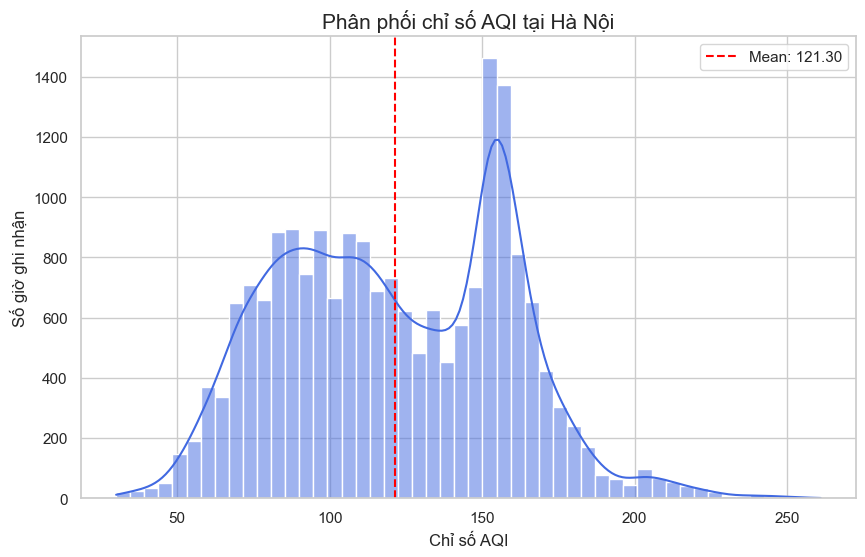
\includegraphics[width=0.72\textwidth]{image/aqitb}
  \caption{Phân phối các mức AQI tại Hà Nội}
  \label{fig:aqi_dist}
\end{figure}

\subsection{Xu hướng theo Năm}

\begin{figure}[H]
  \centering
  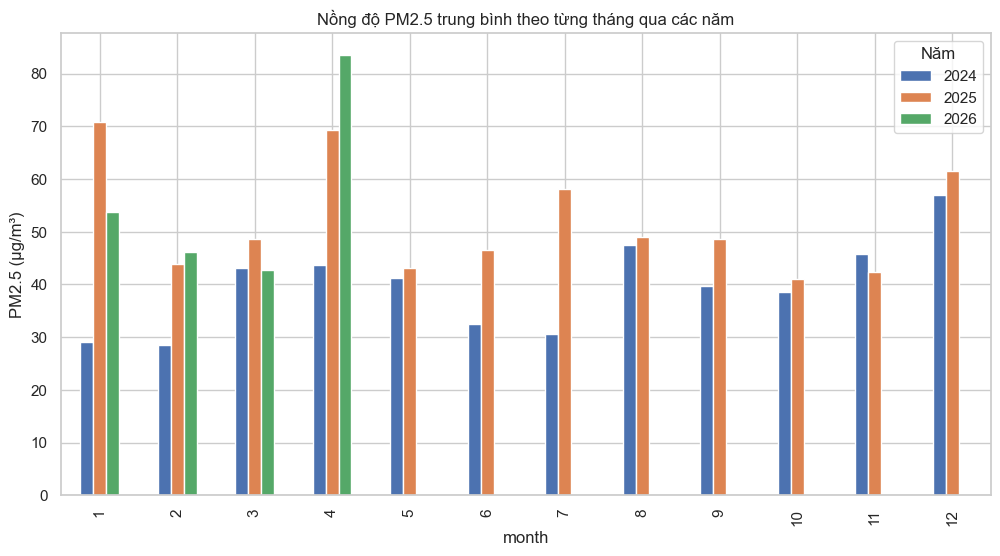
\includegraphics[width=0.85\textwidth]{image/pm2.5tungnam}
  \caption{Xu hướng PM2.5 qua các năm tại Hà Nội}
  \label{fig:pm25_year}
\end{figure}

PM2.5 trung bình biến động theo năm với mùa đông (tháng 12--2) luôn cao hơn mùa hè. Năm 2024 ghi nhận mức ô nhiễm cao bất thường trong giai đoạn tháng 1--2.

\subsection{Biến động theo Giờ trong Ngày}

\begin{figure}[H]
  \centering
  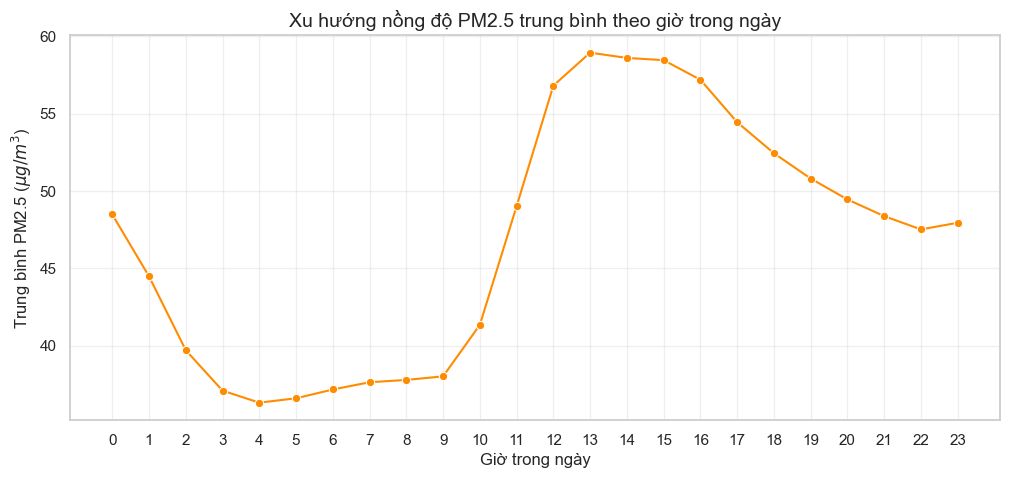
\includegraphics[width=0.8\textwidth]{image/pm2.5trongngay}
  \caption{Biến động PM2.5 theo giờ trong ngày (trung bình)}
  \label{fig:pm25_hour}
\end{figure}

Hai đỉnh ô nhiễm rõ rệt trong ngày:
\begin{itemize}
  \item \textbf{6:00--9:00:} Giờ cao điểm buổi sáng -- giao thông dày đặc kết hợp nghịch nhiệt đêm chưa tan.
  \item \textbf{19:00--22:00:} Giờ cao điểm buổi tối -- đun nấu, đốt rác, giảm gió sau hoàng hôn.
\end{itemize}

Đây là lý do chính để đưa \texttt{hour\_sin} và \texttt{hour\_cos} vào tập đặc trưng.

\subsection{Ảnh hưởng của Mùa}

\begin{figure}[H]
  \centering
  \begin{subfigure}{0.48\textwidth}
    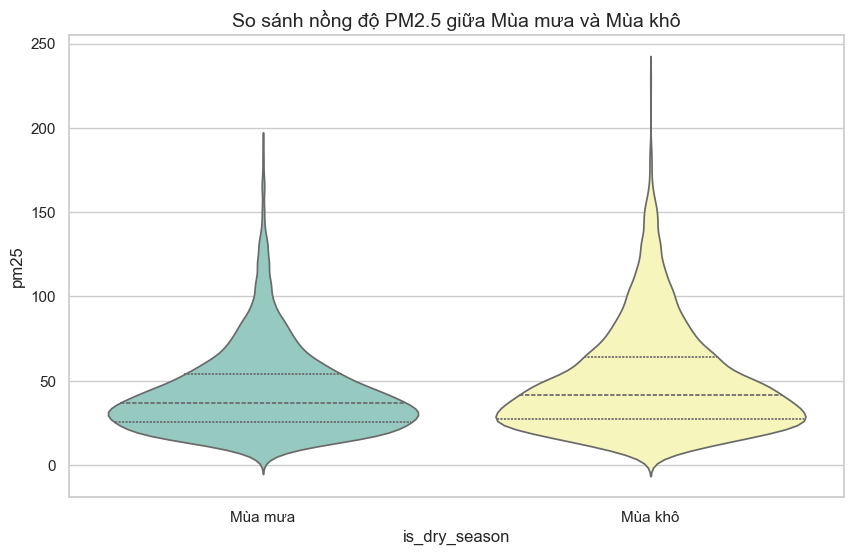
\includegraphics[width=\textwidth]{image/muakho}
    \caption{AQI mùa mưa vs. mùa khô}
  \end{subfigure}
  \hfill
  \begin{subfigure}{0.48\textwidth}
    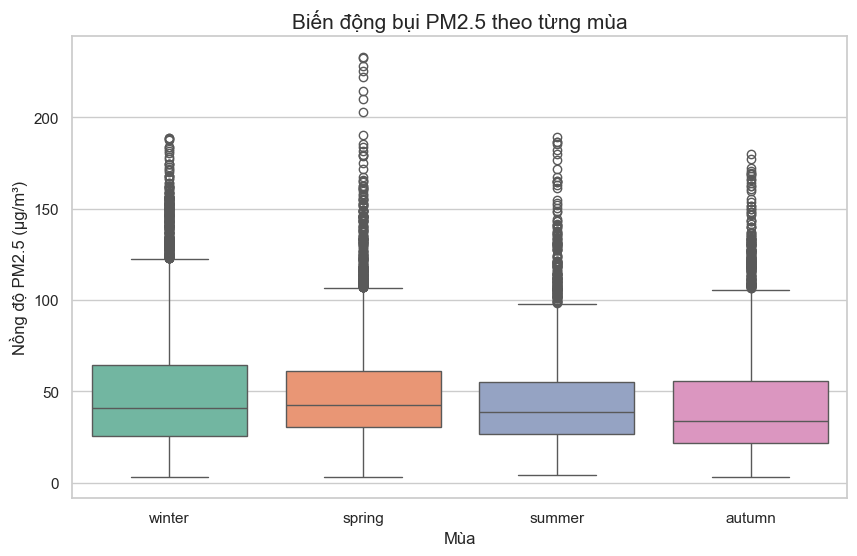
\includegraphics[width=\textwidth]{image/buitheomua}
    \caption{PM2.5 theo mùa}
  \end{subfigure}
  \caption{So sánh ô nhiễm theo mùa tại Hà Nội}
  \label{fig:seasonal}
\end{figure}

Mùa khô (tháng 11--4): PM2.5 và AQI trung bình cao gấp 2--3 lần mùa mưa. Mùa mưa (tháng 5--10): mưa rửa trôi bụi, AQI thường ở mức Tốt đến Trung bình. Biến \texttt{is\_dry\_season} được đưa vào model để nắm bắt sự khác biệt này.

\subsection{Ảnh hưởng của Gió}

\begin{figure}[H]
  \centering
  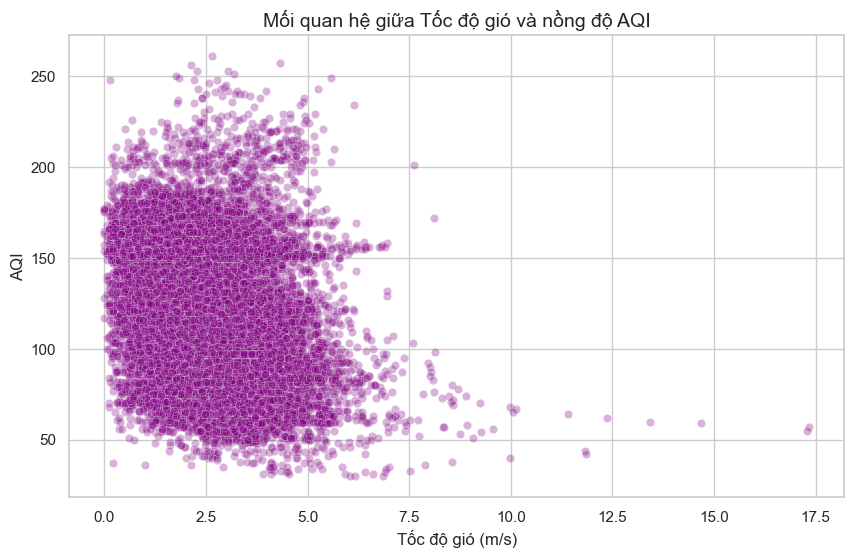
\includegraphics[width=0.75\textwidth]{image/wind+aqi}
  \caption{Mối quan hệ giữa hướng/tốc độ gió và chỉ số AQI}
  \label{fig:wind}
\end{figure}

Gió Bắc và Đông Bắc (thổi từ các khu công nghiệp phía Bắc) thường kéo theo PM2.5 cao hơn; gió Nam kết hợp mưa giúp không khí trong lành hơn. Vì vậy, hướng gió được mã hóa thành hai thành phần vector $(\texttt{wind\_u}, \texttt{wind\_v})$ thay vì dùng góc độ tuần hoàn.

\subsection{Cuối tuần vs. Ngày thường}

\begin{figure}[H]
  \centering
  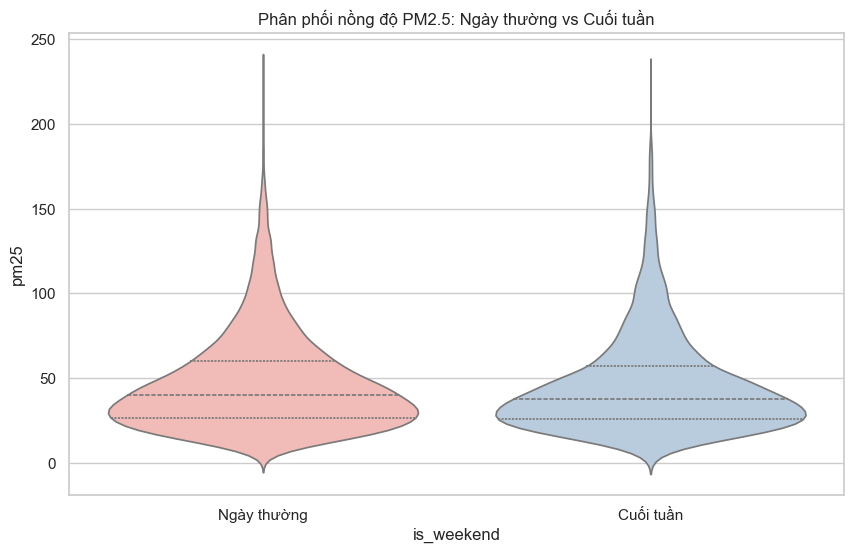
\includegraphics[width=0.7\textwidth]{image/weekend}
  \caption{So sánh AQI ngày thường và cuối tuần}
  \label{fig:weekend}
\end{figure}

AQI vào thứ Bảy, Chủ Nhật thấp hơn khoảng 10--15\% so với ngày trong tuần, phản ánh giảm hoạt động giao thông và công nghiệp. Biến \texttt{is\_weekend} và \texttt{day\_of\_week\_sin/cos} nắm bắt pattern này.

\subsection{Ma trận Tương quan}

\begin{figure}[H]
  \centering
  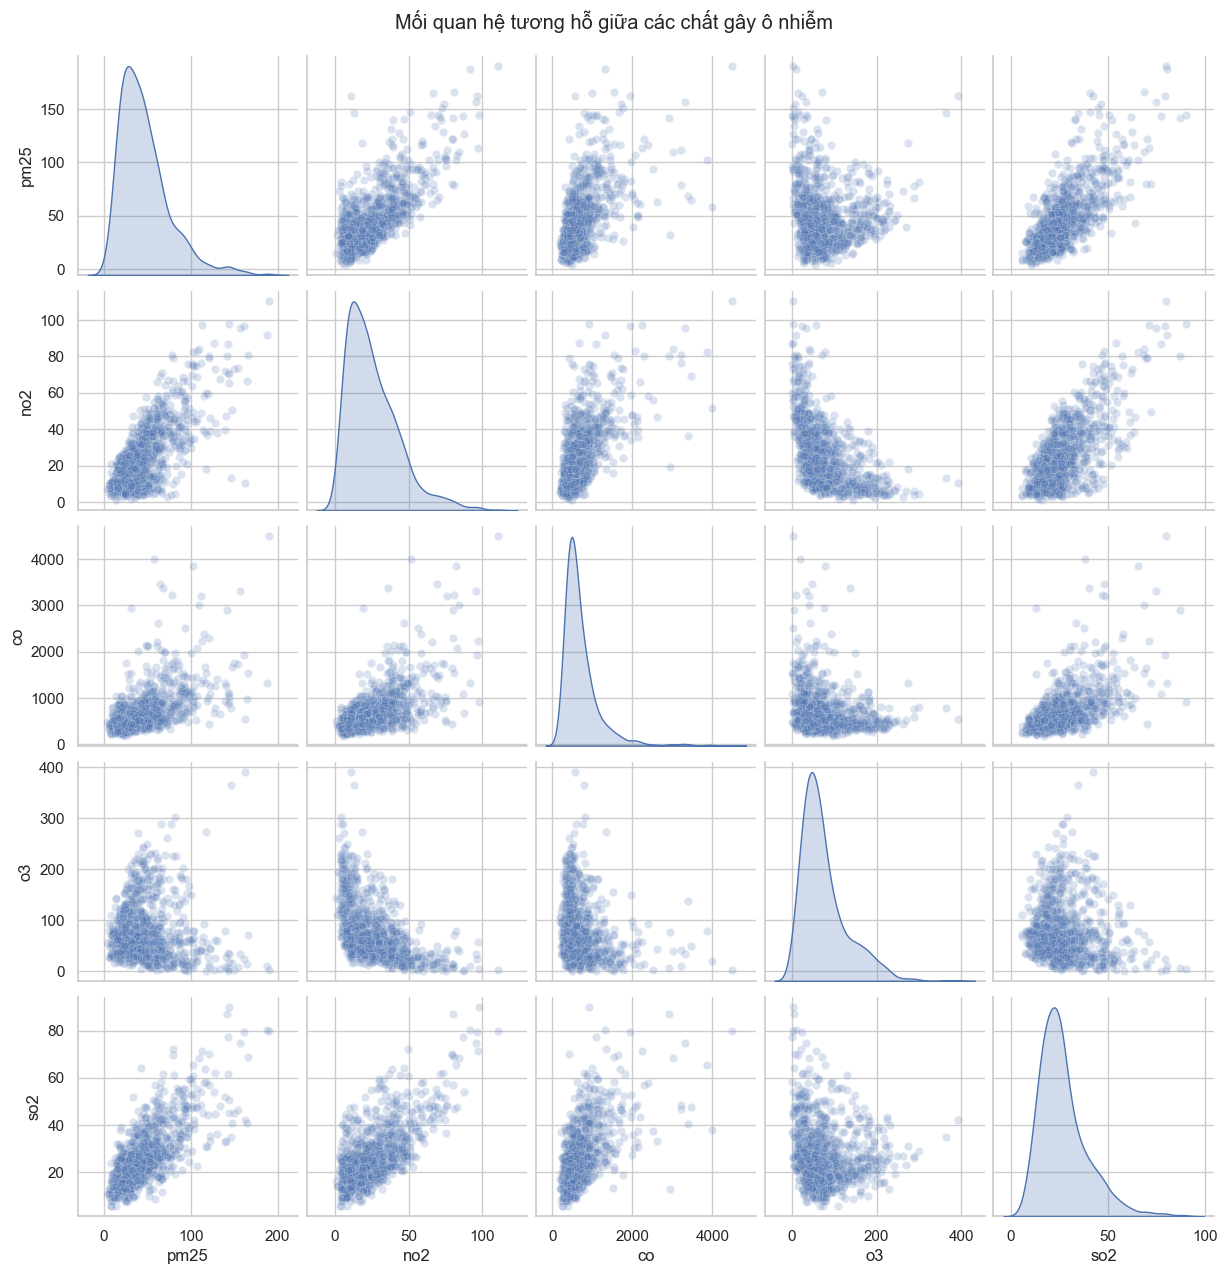
\includegraphics[width=0.8\textwidth]{image/tuongho}
  \caption{Ma trận tương quan giữa các biến chính}
  \label{fig:corr}
\end{figure}

Các quan sát quan trọng từ ma trận tương quan:
\begin{itemize}
  \item PM2.5 và US AQI có tương quan gần hoàn hảo ($r \approx 0{,}98$), xác nhận PM2.5 là chất quyết định AQI tại Hà Nội.
  \item Nhiệt độ tương quan âm với PM2.5 ($r \approx -0{,}45$): ngày nóng thường thoáng hơn.
  \item Tốc độ gió tương quan âm với PM2.5 ($r \approx -0{,}35$): gió thổi phân tán bụi.
  \item Độ ẩm có tương quan dương yếu với PM2.5 trong mùa đông (hiện tượng sương mù ẩm giữ bụi lại).
\end{itemize}

% ============================================================
\chapter{Feature Engineering}
% ============================================================

Feature Engineering là bước quan trọng nhất trong pipeline, chuyển đổi dữ liệu chuỗi thời gian thô thành ma trận đặc trưng phù hợp cho các mô hình học máy phi chuỗi thời gian (MLP, SVR, MARS). Tổng cộng \textbf{145 đặc trưng} được tạo ra.

\section{Đặc trưng Tín hiệu Gốc (Base Signals)}

Bảy biến cơ sở được giữ nguyên và đưa trực tiếp vào mô hình:
\[
  \mathcal{S} = \{\texttt{us\_aqi},\; \texttt{pm25},\; \texttt{pm10},\; \texttt{no2},\; \texttt{o3},\; \texttt{co},\; \texttt{so2}\}
\]
Tổng: \textbf{7 biến}.

\section{Lag Features (Đặc trưng Trễ)}

Với mỗi biến $s \in \mathcal{S}$, giá trị tại các mốc thời gian trước được tạo ra:
\begin{equation}
  \texttt{s\_lag\_kh}(t) = s(t - k), \quad k \in \{1, 3, 6, 12, 24, 168\}
\end{equation}

Lag 168h (1 tuần) là quan trọng nhất vì nắm bắt tính tuần hoàn theo tuần. Hệ thống yêu cầu tối thiểu 170 giờ lịch sử để tính đủ tất cả rolling và lag features.

Với 7 biến tín hiệu × 6 lag bước = \textbf{42 lag signal features}.

Tương tự, 16 biến thời tiết có lag 1h, 3h, 6h: $16 \times 3 = \textbf{48 weather lag features}$.

\section{Rolling Statistics (Thống kê Trượt)}

Với AQI, PM2.5 và PM10, trung bình và độ lệch chuẩn trượt:
\begin{align}
  \texttt{s\_roll\_mean\_wh}(t) &= \frac{1}{w}\sum_{i=0}^{w-1} s(t-i) \\[4pt]
  \texttt{s\_roll\_std\_wh}(t)  &= \sqrt{\frac{1}{w}\sum_{i=0}^{w-1}\!\left(s(t-i) - \overline{s}\right)^2}
\end{align}

với cửa sổ $w \in \{3, 6, 24, 168\}$ giờ ($\texttt{min\_periods} = w$, tức phải đủ dữ liệu mới tính).

Tổng: $3 \times 4 \times 2 = \textbf{24 rolling features}$.

Rolling 168h (trung bình 7 ngày) phản ánh mức nền dài hạn -- giúp phân biệt đợt ô nhiễm đột biến với mức bình thường.

\section{Time Features (Đặc trưng Thời gian)}

Mã hóa chu kỳ (cyclical encoding) tránh bất liên tục tại ranh giới (giờ 23 sang giờ 0):
\begin{align}
  \texttt{hour\_sin}     &= \sin\!\left(\tfrac{2\pi \cdot h}{24}\right), \quad
  \texttt{hour\_cos}      = \cos\!\left(\tfrac{2\pi \cdot h}{24}\right) \\
  \texttt{weekday\_sin}  &= \sin\!\left(\tfrac{2\pi \cdot d}{7}\right), \quad
  \texttt{weekday\_cos}   = \cos\!\left(\tfrac{2\pi \cdot d}{7}\right) \\
  \texttt{month\_sin}    &= \sin\!\left(\tfrac{2\pi \cdot m}{12}\right), \quad
  \texttt{month\_cos}     = \cos\!\left(\tfrac{2\pi \cdot m}{12}\right)
\end{align}

Hai biến nhị phân bổ sung:
\begin{itemize}
  \item \texttt{is\_weekend} = 1 nếu thứ Bảy hoặc Chủ Nhật.
  \item \texttt{is\_dry\_season} = 1 nếu tháng $\in \{11, 12, 1, 2, 3, 4\}$.
\end{itemize}

Tổng: \textbf{8 time features}.

\section{Derived Features (Đặc trưng Phái sinh)}

Các đặc trưng phái sinh từ biến thời tiết:
\begin{align}
  \texttt{wind\_u}       &= -v_w \cdot \sin(\theta_w \cdot \pi/180) \\
  \texttt{wind\_v}       &= -v_w \cdot \cos(\theta_w \cdot \pi/180) \\
  \texttt{temp\_humidity}&= T \times H \\
  \texttt{pressure\_diff}&= P(t) - P(t-1) \\
  \texttt{is\_raining}   &= \mathbf{1}[\texttt{rain}(t) > 0]
\end{align}

Phân tách gió thành hai thành phần vector $(\texttt{wind\_u}, \texttt{wind\_v})$ cho phép mô hình học được hướng gió liên tục thay vì góc độ tuần hoàn, tránh sự nhảy vọt từ 359° sang 0°.

\section{Tổng hợp và Phân chia Dữ liệu}

\begin{table}[H]
\centering
\caption{Tổng hợp 145 đặc trưng theo nhóm}
\label{tab:feature_summary}
\begin{tabular}{llr}
\toprule
\textbf{Nhóm} & \textbf{Mô tả} & \textbf{Số đặc trưng} \\
\midrule
Base signal     & 7 biến ô nhiễm gốc              & 7  \\
Signal lags     & 7 biến × 6 lag bước             & 42 \\
Rolling stats   & 3 biến × 4 cửa sổ × 2 thống kê  & 24 \\
Weather raw     & 16 biến khí tượng               & 16 \\
Weather lags    & 16 biến × 3 lag bước            & 48 \\
Time features   & sin/cos giờ, ngày, tháng + 2 cờ  & 8  \\
\midrule
\textbf{Tổng}   & & \textbf{145} \\
\bottomrule
\end{tabular}
\end{table}

Dữ liệu được phân chia theo thứ tự thời gian (chronological split) để tránh data leakage:
\begin{equation}
  \underbrace{\text{Train (70\%)}}_{\approx 13{,}800\;\text{giờ}} \;\Big|\;
  \underbrace{\text{Validation (10\%)}}_{\approx 1{,}970\;\text{giờ}} \;\Big|\;
  \underbrace{\text{Test (20\%)}}_{\approx 3{,}940\;\text{giờ}}
\end{equation}

Quy trình: hyperparameter search trên Validation, retrain trên Train+Validation, đánh giá cuối trên Test.

% ============================================================
\chapter{Phương pháp và Mô hình}
% ============================================================

\section{Baseline: Persistence Model}

Mô hình baseline đơn giản nhất -- dự báo AQI tương lai bằng AQI hiện tại:
\begin{equation}
  \hat{y}(t+h) = y(t)
\end{equation}

Baseline phản ánh ``quán tính'' của chuỗi AQI. Ở horizon +1h, baseline đã khá tốt (AQI thay đổi chậm); ở +24h, baseline kém đáng kể do AQI có thể thay đổi hoàn toàn trong một ngày.

\section{ARIMA}

ARIMA$(p, d, q)$ mô hình hóa chuỗi US AQI univariate:
\begin{equation}
  \Phi(B)(1-B)^d y_t = \Theta(B)\varepsilon_t
\end{equation}
với $B$ là toán tử trễ, $\Phi(B) = 1 - \phi_1 B - \cdots - \phi_p B^p$, $\Theta(B) = 1 + \theta_1 B + \cdots + \theta_q B^q$.

\textbf{Chọn order:} Grid search trên $p \leq 3$, $d \leq 1$, $q \leq 3$, chọn theo AIC tối thiểu. Order tốt nhất là ARIMA(3,0,3).

\textbf{Đánh giá:} Rolling-origin forecast -- tại mỗi điểm test, mô hình được cập nhật bằng \texttt{model.append([actual])} trước khi dự báo $h$ bước tới. Giới hạn: univariate, không khai thác thời tiết.

\section{VARMA/VARMAX}

VARMA$(p, q)$ mở rộng ARIMA sang đa biến với vector:
\[
  \mathbf{y}_t = [\text{US AQI}, \text{PM2.5}, \text{PM10}, \text{NO}_2, \text{O}_3, \text{CO}, \text{SO}_2]^\top
\]

\begin{equation}
  \mathbf{y}_t = \mathbf{c} + \sum_{i=1}^{p}\mathbf{\Phi}_i \mathbf{y}_{t-i} + \sum_{j=1}^{q}\mathbf{\Theta}_j \boldsymbol{\varepsilon}_{t-j} + \boldsymbol{\varepsilon}_t
\end{equation}

Chuỗi được chuẩn hóa StandardScaler trước khi fitting và nghịch chuẩn sau dự báo. Order chọn theo AIC trên grid $p \leq 2$, $q \leq 1$.

\section{MLP (Multilayer Perceptron)}

MLP với pipeline StandardScaler $\to$ MLPRegressor:

\begin{itemize}
  \item \textbf{Kiến trúc grid search:} Hidden layers $(64,)$, $(128,)$, $(64, 32)$
  \item \textbf{Regularization:} $\alpha \in \{10^{-4}, 10^{-3}\}$ (L2)
  \item \textbf{Optimizer:} Adam, learning rate $0{,}001$
  \item \textbf{Early stopping:} 10\% validation split, 20 iter không cải thiện
  \item \textbf{Max iterations:} 500
\end{itemize}

Hàm kích hoạt ReLU. Mô hình tốt nhất theo validation RMSE được retrain trên Train+Val.

\section{SVMR (Support Vector Machine Regression)}

SVR với kernel RBF tối thiểu hóa:
\begin{equation}
  \min_{\mathbf{w}, b, \xi} \; \frac{1}{2}\|\mathbf{w}\|^2 + C\sum_{i=1}^n (\xi_i + \xi_i^*)
  \quad \text{s.t.} \quad |y_i - f(\mathbf{x}_i)| \leq \epsilon + \xi_i
\end{equation}

\textbf{Grid search:} $C \in \{1, 10, 100\}$, $\epsilon \in \{0{,}1, 1{,}0, 2{,}0\}$, gamma = \texttt{scale}.

Pipeline: StandardScaler $\to$ SVR. SVMR ổn định ở horizon dài nhờ regularization mạnh giảm overfitting trên tập đặc trưng 145 chiều.

\section{MARS (Multivariate Adaptive Regression Splines)}

MARS xây dựng hàm hồi quy dạng tổ hợp hinge functions:
\begin{equation}
  f(\mathbf{x}) = \beta_0 + \sum_{m=1}^{M} \beta_m \prod_{k=1}^{K_m} H\!\left[s_{km}(x_{v(k,m)} - t_{km})\right]
\end{equation}

với $H(z) = \max(0, z)$, $t_{km}$ là knot, $s_{km} \in \{-1, +1\}$ là hướng.

Forward pass tự động tìm knots; backward pass loại knots kém (GCV pruning).

\textbf{Grid search:} max\_terms $\in \{30, 60, 90\}$, max\_degree $\in \{1, 2\}$, penalty $\in \{2{,}0, 3{,}0\}$.

Thư viện: \texttt{py-earth2} (Python). MARS vượt trội ở horizon +1h nhờ khả năng nắm bắt phi tuyến cục bộ tinh tế.

\section{Quy trình Huấn luyện Tổng quát}

\begin{figure}[H]
\centering
\begin{tikzpicture}[
  box/.style={rectangle, draw=headerblue, fill=blue!8, rounded corners=4pt,
              text width=3cm, align=center, minimum height=1cm, font=\small},
  arr/.style={-{Stealth[length=2.5mm]}, thick, color=headerblue}
]
  \node[box] (data)    {Dữ liệu\\training};
  \node[box] (feat)    [right=1cm of data]   {Feature\\Engineering};
  \node[box] (split)   [right=1cm of feat]   {Train/Val/Test\\Split};
  \node[box] (grid)    [right=1cm of split]  {Grid Search\\(Val RMSE)};
  \node[box] (retrain) [right=1cm of grid]   {Retrain\\Train+Val};
  \node[box] (eval)    [right=1cm of retrain]{Đánh giá\\Test set};

  \draw[arr] (data)    -- (feat);
  \draw[arr] (feat)    -- (split);
  \draw[arr] (split)   -- (grid);
  \draw[arr] (grid)    -- (retrain);
  \draw[arr] (retrain) -- (eval);
\end{tikzpicture}
\caption{Quy trình huấn luyện và chọn mô hình}
\label{fig:train_pipeline}
\end{figure}

Tại mỗi horizon, model tốt nhất (RMSE test nhỏ nhất) được lưu vào \texttt{outputs/gijon\_aqi\_hourly/models/} và đăng ký trong \texttt{best\_models.json} để inference.

% ============================================================
\chapter{Kết quả và Đánh giá}
% ============================================================

\section{Các Độ đo Đánh giá}

\begin{itemize}
  \item \textbf{MAE:} $\displaystyle\frac{1}{n}\sum|y_i - \hat{y}_i|$ -- sai số tuyệt đối trung bình (AQI).
  \item \textbf{RMSE:} $\displaystyle\sqrt{\frac{1}{n}\sum(y_i - \hat{y}_i)^2}$ -- nhạy hơn với sai số lớn.
  \item \textbf{$R^2$:} $\displaystyle 1 - \frac{\text{SS}_\text{res}}{\text{SS}_\text{tot}}$ -- tỷ lệ phương sai giải thích được.
  \item \textbf{Class Accuracy:} Độ chính xác phân loại 6 mức AQI -- đánh giá tính hữu dụng thực tế.
\end{itemize}

Mọi dự báo được clip vào $[0, 500]$ trước khi tính metric.

\section{Kết quả Tổng hợp}

\begin{table}[H]
\centering
\caption{Kết quả đánh giá toàn bộ mô hình trên tập Test}
\label{tab:results_full}
\begin{tabular}{clrrrr}
\toprule
\textbf{Horizon} & \textbf{Mô hình} & \textbf{MAE} & \textbf{RMSE} & \textbf{$R^2$} & \textbf{Class Acc.} \\
\midrule
\rowcolor{green!12}
+1h & \textbf{MARS} $\star$ & \textbf{1.22} & \textbf{2.28} & \textbf{0.9964} & \textbf{97.5\%} \\
+1h & ARIMA         & 1.26 & 2.60  & 0.9952 & 97.3\% \\
+1h & Persistence   & 1.74 & 3.67  & 0.9905 & 96.7\% \\
+1h & MLP           & 3.50 & 4.62  & 0.9850 & 93.2\% \\
+1h & SVMR          & 2.77 & 5.02  & 0.9823 & 94.0\% \\
\midrule
\rowcolor{green!12}
+6h & \textbf{SVMR} $\star$ & \textbf{4.89} & \textbf{7.42} & \textbf{0.9613} & \textbf{89.2\%} \\
+6h & MLP           & 5.94 & 7.73  & 0.9580 & 88.2\% \\
+6h & MARS          & 6.04 & 7.88  & 0.9564 & 87.1\% \\
+6h & Persistence   & 9.43 & 15.53 & 0.8306 & 82.4\% \\
\midrule
\rowcolor{green!12}
+24h & \textbf{SVMR} $\star$ & \textbf{17.11} & \textbf{21.95} & \textbf{0.6614} & \textbf{61.7\%} \\
+24h & MARS          & 17.36 & 22.45 & 0.6456 & 62.4\% \\
+24h & Persistence   & 22.96 & 30.91 & 0.3282 & 60.0\% \\
\bottomrule
\multicolumn{6}{l}{\small $\star$ = mô hình được chọn cho production tại horizon đó}
\end{tabular}
\end{table}

\section{Phân tích theo Horizon}

\subsection{Horizon +1h: MARS đạt kết quả xuất sắc}

Ở horizon ngắn, AQI có tính tự tương quan rất cao. MARS tận dụng tốt điều này nhờ hinge functions nắm bắt quan hệ phi tuyến cục bộ tinh tế.

\begin{itemize}
  \item $R^2 = 0{,}9964$: 99.64\% phương sai được giải thích.
  \item RMSE = 2.28 AQI: sai số trung bình chỉ hơn 2 đơn vị AQI.
  \item Cả MARS và ARIMA đều vượt đáng kể Persistence, cho thấy lag features cung cấp thông tin cận biên có giá trị.
  \item MLP và SVMR kém hơn MARS và ARIMA ở +1h do thiếu cơ chế khai thác tính cục bộ mạnh.
\end{itemize}

\subsection{Horizon +6h: SVMR ổn định}

Ở 6 giờ tới, tính tự tương quan giảm và mô hình cần khai thác nhiều thông tin phụ trợ. SVMR với regularization mạnh tránh overfitting tốt hơn trên không gian 145 chiều.

\begin{itemize}
  \item SVMR: $R^2 = 0{,}9613$ -- rất tốt cho kế hoạch trong ngày.
  \item Khoảng cách SVMR/MLP/MARS rất nhỏ ($\Delta$RMSE $< 0{,}5$ AQI), cả ba đều cạnh tranh.
  \item Persistence giảm mạnh xuống $R^2 = 0{,}83$, xác nhận giá trị của các mô hình ML.
\end{itemize}

\subsection{Horizon +24h: Thách thức dự báo dài hạn}

\begin{itemize}
  \item SVMR: $R^2 = 0{,}6614$ -- vẫn hữu ích cho cảnh báo sớm mặc dù uncertainty lớn.
  \item MARS có class accuracy cao hơn SVMR (62.4\% vs 61.7\%) nhưng RMSE cao hơn.
  \item Cả hai vượt Persistence đáng kể ($R^2 = 0{,}33$).
\end{itemize}

\section{Phân tích Phân loại Mức AQI}

\begin{table}[H]
\centering
\caption{Độ chính xác phân loại 6 mức AQI (mô hình tốt nhất mỗi horizon)}
\label{tab:class_acc}
\begin{tabular}{lrrr}
\toprule
\textbf{Horizon} & \textbf{Mô hình} & \textbf{Class Accuracy} & \textbf{Macro F1} \\
\midrule
+1h  & MARS & \good{97.5\%} & 0.956 \\
+6h  & SVMR & \warn{89.2\%} & 0.822 \\
+24h & SVMR & \bad{61.7\%}  & 0.466 \\
\bottomrule
\end{tabular}
\end{table}

Với độ chính xác phân loại 97.5\% tại +1h, hệ thống đủ tin cậy để cung cấp cảnh báo mức AQI cho người dùng. Tại +24h, 61.7\% vẫn có giá trị thực tiễn -- cao hơn ngưỡng random (1/6 $\approx$ 16.7\%) rất nhiều và đặc biệt hữu ích cho phân loại nhị phân ``an toàn'' (AQI $\leq$ 100) vs. ``nguy hiểm'' (AQI $>$ 100) với độ chính xác cao hơn nhiều.

\section{Nhận xét Tổng quan}

\begin{enumerate}
  \item Tất cả mô hình ML (MARS, SVMR, MLP) vượt Baseline Persistence ở cả ba horizon -- xác nhận giá trị của 145 đặc trưng được tạo ra.
  \item MARS phù hợp hơn cho dự báo ngắn hạn; SVMR ổn định hơn ở horizon dài.
  \item Feature Engineering (đặc biệt lag 168h và rolling 168h) là yếu tố then chốt giúp ML vượt ARIMA ở horizon dài.
  \item Có thể cải thiện thêm bằng LSTM hoặc Temporal Fusion Transformer nếu có đủ tài nguyên.
\end{enumerate}

% ============================================================
\chapter{Triển khai Hệ thống}
% ============================================================

\section{Kiến trúc Tổng quát}

\begin{figure}[H]
\centering
\begin{tikzpicture}[
  comp/.style={rectangle, draw=headerblue, fill=blue!8, rounded corners=5pt,
               text width=3.2cm, align=center, minimum height=1.2cm, font=\small},
  api/.style={ellipse, draw=gray!70, fill=gray!10, text width=2.8cm,
              align=center, minimum height=1cm, font=\small},
  arr/.style={-{Stealth[length=2.5mm]}, thick, color=headerblue},
  label/.style={font=\tiny, color=gray}
]
  \node[api]  (omapi) {Open-Meteo\\Air + Weather API};
  \node[comp] (be)    [right=1.4cm of omapi] {FastAPI\\Backend};
  \node[comp] (ml)    [above=0.9cm of be]    {ML Models\\MARS / SVMR};
  \node[comp] (fe)    [right=1.4cm of be]    {Web\\Frontend (JS)};
  \node[api]  (user)  [right=1.4cm of fe]    {Người\\dùng};

  \draw[arr] (omapi) -- node[below, label]{JSON hourly} (be);
  \draw[arr] (be.north) -- node[right, label]{features} (ml.south);
  \draw[arr] (ml.south) -- node[left, label]{pred} (be.north);
  \draw[arr] (be) -- node[below, label]{JSON API} (fe);
  \draw[arr] (fe) -- (user);
\end{tikzpicture}
\caption{Kiến trúc hệ thống AirSense Hà Nội}
\label{fig:architecture}
\end{figure}

\section{Backend API (FastAPI)}

\subsection{Các Endpoint}

\begin{table}[H]
\centering
\caption{Danh sách API endpoints}
\label{tab:endpoints}
\begin{tabularx}{\textwidth}{llX}
\toprule
\textbf{Method} & \textbf{Endpoint} & \textbf{Mô tả} \\
\midrule
GET & \texttt{/}             & Phục vụ Web UI (index.html) \\
GET & \texttt{/api/forecast} & Trả về dự báo AQI live (3 horizons) \\
GET & \texttt{/api/health}   & Kiểm tra trạng thái, danh sách models \\
GET & \texttt{/api/metrics}  & Kết quả đánh giá mô hình chi tiết \\
\bottomrule
\end{tabularx}
\end{table}

\subsection{Pipeline Suy luận (Inference)}

Khi nhận request \texttt{GET /api/forecast?history\_days=10}, backend thực hiện:

\begin{enumerate}
  \item \textbf{Lấy dữ liệu live:} Gọi song song Air Quality API và Weather API với \texttt{past\_days=10}, \texttt{forecast\_days=1}. Retry tối đa 3 lần.
  \item \textbf{Merge và lọc:} Merge theo \texttt{datetime}, lọc $\leq$ thời điểm hiện tại UTC.
  \item \textbf{Derived features:} Tính \texttt{wind\_u/v}, \texttt{temp\_humidity}, \texttt{pressure\_diff}, \texttt{is\_raining}. Nội suy NaN tối đa 3 bước.
  \item \textbf{Feature Engineering:} Gọi \texttt{add\_time\_features()} và \texttt{add\_lag\_and\_rolling\_features()} -- giống hệt pipeline training.
  \item \textbf{Prediction:} Với mỗi horizon $h$, lấy hàng cuối (sau khi loại NaN) và gọi \texttt{model.predict([row])}.
  \item \textbf{Format response:} AQI hiện tại, 3 dự báo kèm khoảng tin cậy ($\pm$ RMSE), 72h quan sát gần nhất.
\end{enumerate}

\textbf{Model caching:} Tất cả model được load vào RAM lần đầu và cache trong \texttt{\_MODEL\_CACHE}, tránh I/O lặp lại giữa các request.

\subsection{Khoảng Tin cậy}

Khoảng tin cậy được tính đơn giản dựa trên RMSE của mô hình trên tập test:
\begin{align}
  \text{AQI\_low}  &= \max(0,\; \hat{y}(t+h) - \text{RMSE}_h) \\
  \text{AQI\_high} &= \min(500,\; \hat{y}(t+h) + \text{RMSE}_h)
\end{align}

\section{Frontend Web Application}

Frontend xây dựng bằng Vanilla JavaScript, HTML5 và CSS3 (không framework).

\textbf{Tính năng chính:}
\begin{itemize}
  \item \textbf{AQI card hiện tại:} Màu nền động theo mức độ ô nhiễm (xanh/vàng/cam/đỏ/tím/nâu).
  \item \textbf{Chi tiết chất ô nhiễm:} PM2.5, PM10, NO$_2$, O$_3$ cùng nhiệt độ, độ ẩm, gió.
  \item \textbf{3 thẻ dự báo:} +1h, +6h, +24h với giá trị AQI, khoảng tin cậy và model sử dụng.
  \item \textbf{Biểu đồ đường 72h:} Lịch sử AQI và PM2.5 theo thời gian (Chart.js).
  \item \textbf{Khuyến nghị sức khỏe:} Tùy chỉnh theo mức AQI hiện tại với 6 mức lời khuyên cụ thể.
  \item \textbf{Dark mode + Responsive design:} Tối ưu cho cả desktop và mobile.
\end{itemize}

\section{Cấu trúc Thư mục Dự án}

\begin{lstlisting}[language=bash, caption={Cấu trúc thư mục dự án}]
Data-Science/
|-- app/
|   +-- main.py             # FastAPI backend (inference + API endpoints)
|-- scripts/
|   +-- train_gijon_aqi_hourly.py  # Training pipeline (5 models x 3 horizons)
|-- data/
|   |-- raw/air_quality/    # CSV raw theo tháng
|   |-- raw/weather/        # CSV raw theo tháng
|   +-- processed/          # ML-ready datasets
|-- outputs/
|   +-- gijon_aqi_hourly/
|       |-- models/         # .joblib / .pkl models
|       |-- metadata/       # feature_cols, best params
|       |-- predictions/    # y_true vs y_pred CSV
|       +-- reports/        # metrics.csv, best_models.json
|-- image/                  # Hình ảnh EDA
|-- build_hanoi_dataset.py  # Thu thập dữ liệu tự động
|-- index.html              # Frontend UI
+-- requirements.txt
\end{lstlisting}

\section{Hướng dẫn Cài đặt và Chạy}

\begin{lstlisting}[language=bash, caption={Cài đặt và chạy AirSense Hà Nội}]
# 1. Clone repository
git clone https://github.com/nguyenquypro17/Data-Science.git
cd Data-Science

# 2. Cài đặt phụ thuộc
pip install -r requirements.txt

# 3. Thu thập dữ liệu (lần đầu)
python build_hanoi_dataset.py

# 4. Training (khoảng 30-60 phút tùy máy)
python scripts/train_gijon_aqi_hourly.py \
  --horizons 1 6 24 \
  --train-ratio 0.70 --val-ratio 0.10 --test-ratio 0.20 \
  --allow-skip-mars-if-missing

# 5. Chạy API server
uvicorn app.main:app --host 0.0.0.0 --port 8000 --reload

# 6. Mở trình duyệt: http://localhost:8000
\end{lstlisting}

% ============================================================
\chapter{Kết luận và Hướng Phát triển}
% ============================================================

\section{Tóm tắt Kết quả Đạt được}

Dự án AirSense Hà Nội đã hoàn thành thành công toàn bộ các mục tiêu đề ra:

\begin{enumerate}
  \item \textbf{Thu thập dữ liệu:} Pipeline tự động thu thập dữ liệu chất lượng không khí và khí tượng theo giờ từ Open-Meteo, tạo ra $\approx 19{,}700$ điểm dữ liệu.
  \item \textbf{EDA:} Phát hiện các pattern quan trọng -- hai đỉnh ô nhiễm trong ngày (sáng/tối), chênh lệch mùa khô/mưa 2--3x, ảnh hưởng của gió và cuối tuần.
  \item \textbf{Feature Engineering:} Tạo 145 đặc trưng, với lag 168h và rolling 168h là yếu tố then chốt.
  \item \textbf{Kết quả mô hình:}
    \begin{itemize}
      \item MARS: $R^2 = 0{,}9964$, RMSE = 2.28 AQI tại +1h (97.5\% class accuracy).
      \item SVMR: $R^2 = 0{,}9613$, RMSE = 7.42 AQI tại +6h (89.2\% class accuracy).
      \item SVMR: $R^2 = 0{,}6614$, RMSE = 21.95 AQI tại +24h (61.7\% class accuracy).
    \end{itemize}
  \item \textbf{Triển khai:} Web Application hoàn chỉnh với FastAPI backend và JavaScript frontend, cung cấp dự báo thời gian thực kèm khuyến nghị sức khỏe.
\end{enumerate}

\section{Hạn chế}

\begin{itemize}
  \item \textbf{Không có dữ liệu giao thông:} Lưu lượng phương tiện là yếu tố ô nhiễm quan trọng nhưng chưa được đưa vào mô hình.
  \item \textbf{Một điểm đo duy nhất:} Chỉ dùng tọa độ trung tâm Hà Nội; ô nhiễm khác nhau giữa các quận.
  \item \textbf{Horizon +24h còn hạn chế:} $R^2 = 0{,}66$ phản ánh uncertainty lớn khi dự báo dài hạn.
  \item \textbf{Chưa có retraining tự động:} Mô hình không tự cập nhật, có thể bị drift theo thời gian.
  \item \textbf{Khoảng tin cậy đơn giản:} Dùng $\pm$RMSE thay vì conformal prediction hoặc Bayesian intervals.
\end{itemize}

\section{Hướng Phát triển}

\begin{itemize}
  \item \textbf{Deep Learning:} Thử nghiệm LSTM, Transformer (Temporal Fusion Transformer) -- kỳ vọng cải thiện horizon +24h.
  \item \textbf{Dữ liệu giao thông:} Tích hợp API Google Maps Traffic để bổ sung biến lưu lượng xe theo giờ.
  \item \textbf{Nhiều trạm đo:} Thu thập dữ liệu từ nhiều điểm để tạo bản đồ ô nhiễm không gian-thời gian.
  \item \textbf{Retraining tự động:} CI/CD pipeline với schedule retraining hàng tuần, tự động cập nhật model tốt nhất.
  \item \textbf{Conformal Prediction:} Khoảng tin cậy có đảm bảo thống kê thay vì $\pm$RMSE đơn giản.
  \item \textbf{Mở rộng địa lý:} Áp dụng pipeline tương tự cho TP.HCM, Đà Nẵng.
  \item \textbf{Mobile App:} Ứng dụng di động với push notification khi AQI vượt ngưỡng.
  \item \textbf{SHAP values:} Giải thích mô hình -- tại sao mô hình dự báo một giá trị AQI cụ thể.
\end{itemize}

% ============================================================
\chapter*{Tài liệu Tham khảo}
\addcontentsline{toc}{chapter}{Tài liệu Tham khảo}
% ============================================================

\begin{thebibliography}{99}

\bibitem{benali2019predicting}
Benali, L., Notton, G., Fouilloy, A., Voyant, C., \& Dizene, R. (2019).
\textit{Solar radiation forecasting using artificial neural network and random forest methods: Application to normal beam, horizontal diffuse and global components}.
\textit{Renewable Energy}, 132, 871--884.

\bibitem{li2017long}
Li, X., Peng, L., Yao, X., Cui, S., Hu, Y., You, C., \& Chi, T. (2017).
\textit{Long short-term memory neural network for air pollutant concentration predictions: Method development and evaluation}.
\textit{Environmental Pollution}, 231, 997--1004.

\bibitem{friedman1991multivariate}
Friedman, J. H. (1991).
\textit{Multivariate Adaptive Regression Splines}.
\textit{The Annals of Statistics}, 19(1), 1--67.

\bibitem{box1976time}
Box, G. E. P., Jenkins, G. M., \& Reinsel, G. C. (2015).
\textit{Time Series Analysis: Forecasting and Control} (5th ed.).
Wiley.

\bibitem{vapnik1995nature}
Vapnik, V. N. (1995).
\textit{The Nature of Statistical Learning Theory}.
Springer, New York.

\bibitem{sims1980macroeconomics}
Sims, C. A. (1980).
\textit{Macroeconomics and Reality}.
\textit{Econometrica}, 48(1), 1--48.

\bibitem{openmeteo}
Open-Meteo (2024).
\textit{Open-Meteo: Free Weather API for non-commercial use}.
\url{https://open-meteo.com}. Truy cập tháng 6/2025.

\bibitem{usepaaqi}
U.S. Environmental Protection Agency (2024).
\textit{AQI Basics}.
\url{https://www.airnow.gov/aqi/aqi-basics/}. Truy cập tháng 6/2025.

\bibitem{fastapi}
Ramírez, S. (2024).
\textit{FastAPI: Modern, fast web framework for building APIs with Python}.
\url{https://fastapi.tiangolo.com}. Truy cập tháng 6/2025.

\bibitem{scikit}
Pedregosa, F., et al. (2011).
\textit{Scikit-learn: Machine Learning in Python}.
\textit{Journal of Machine Learning Research}, 12, 2825--2830.

\end{thebibliography}

% ============================================================
\appendix
\chapter{Data Dictionary -- Danh sách Biến}

\begin{table}[H]
\centering
\caption{Data dictionary đầy đủ các biến trong bộ dữ liệu}
\label{tab:data_dict_full}
\small
\begin{tabular}{llll}
\toprule
\textbf{Biến} & \textbf{Kiểu} & \textbf{Đơn vị} & \textbf{Mô tả} \\
\midrule
\texttt{datetime}           & datetime64 & UTC    & Dấu thời gian (UTC) \\
\texttt{us\_aqi}            & float64    & --     & US AQI (biến mục tiêu) \\
\texttt{pm25}               & float64    & µg/m³  & Nồng độ PM2.5 \\
\texttt{pm10}               & float64    & µg/m³  & Nồng độ PM10 \\
\texttt{no2}                & float64    & µg/m³  & Nitrogen dioxide \\
\texttt{o3}                 & float64    & µg/m³  & Ozone \\
\texttt{co}                 & float64    & µg/m³  & Carbon monoxide \\
\texttt{so2}                & float64    & µg/m³  & Sulphur dioxide \\
\texttt{temperature}        & float64    & °C     & Nhiệt độ 2m \\
\texttt{humidity}           & float64    & \%     & Độ ẩm tương đối \\
\texttt{dew\_point}         & float64    & °C     & Nhiệt độ điểm sương \\
\texttt{pressure\_msl}      & float64    & hPa    & Áp suất mực nước biển \\
\texttt{surface\_pressure}  & float64    & hPa    & Áp suất bề mặt \\
\texttt{wind\_speed}        & float64    & m/s    & Tốc độ gió 10m \\
\texttt{wind\_direction}    & float64    & độ     & Hướng gió \\
\texttt{wind\_gusts}        & float64    & m/s    & Gió giật 10m \\
\texttt{precipitation}      & float64    & mm     & Tổng lượng mưa \\
\texttt{rain}               & float64    & mm     & Lượng mưa (không tuyết) \\
\texttt{cloud\_cover}       & float64    & \%     & Độ che phủ mây \\
\texttt{wind\_u}            & float64    & m/s    & Thành phần gió U (Đông-Tây) \\
\texttt{wind\_v}            & float64    & m/s    & Thành phần gió V (Bắc-Nam) \\
\texttt{temp\_humidity}     & float64    & --     & Tích nhiệt độ × độ ẩm \\
\texttt{pressure\_diff}     & float64    & hPa    & Biến thiên áp suất theo giờ \\
\texttt{is\_raining}        & int64      & 0/1    & Cờ đang mưa \\
\texttt{is\_weekend}        & int64      & 0/1    & Cờ cuối tuần \\
\texttt{is\_dry\_season}    & int64      & 0/1    & Cờ mùa khô (tháng 11--4) \\
\texttt{hour\_sin/cos}      & float64    & --     & Mã hóa chu kỳ giờ \\
\texttt{weekday\_sin/cos}   & float64    & --     & Mã hóa chu kỳ ngày trong tuần \\
\texttt{month\_sin/cos}     & float64    & --     & Mã hóa chu kỳ tháng \\
\bottomrule
\end{tabular}
\end{table}

\chapter{Ví dụ JSON Response API}

\begin{lstlisting}[language=Python, caption={Mẫu JSON response GET /api/forecast}]
{
  "location": {
    "name": "Ha Noi",
    "latitude": 21.0285,
    "longitude": 105.8542,
    "timezone": "Asia/Bangkok"
  },
  "current": {
    "time_local": "2025-06-09T14:00:00+07:00",
    "us_aqi": 92.0,
    "category": {
      "key": "moderate",
      "label": "Trung binh",
      "color": "#f2c94c",
      "severity": "watch",
      "advice": "Nguoi nhay cam nen giam hoat dong ngoai troi keo dai."
    },
    "pm25": 38.5, "pm10": 55.2,
    "temperature": 32.1, "humidity": 68.0, "wind_speed": 2.3
  },
  "forecasts": [
    {
      "horizon_hours": 1, "model": "MARS",
      "aqi": 95.3, "aqi_low": 93.0, "aqi_high": 97.6,
      "target_time_local": "2025-06-09T15:00:00+07:00",
      "metrics": {"rmse": 2.28, "mae": 1.22, "r2": 0.9964}
    },
    {
      "horizon_hours": 6, "model": "SVMR",
      "aqi": 110.1, "aqi_low": 102.7, "aqi_high": 117.5,
      "target_time_local": "2025-06-09T20:00:00+07:00",
      "metrics": {"rmse": 7.42, "mae": 4.89, "r2": 0.9613}
    },
    {
      "horizon_hours": 24, "model": "SVMR",
      "aqi": 135.0, "aqi_low": 113.1, "aqi_high": 156.9,
      "target_time_local": "2025-06-10T14:00:00+07:00",
      "metrics": {"rmse": 21.95, "mae": 17.11, "r2": 0.6614}
    }
  ],
  "recent_observations": [
    {"time_local": "2025-06-09T12:00:00+07:00", "us_aqi": 88.0, ...},
    ...
  ]
}
\end{lstlisting}

\end{document}
